% !TEX root = ../my-thesis.tex
%
\chapter{Related Work}
\label{sec:related}

\section{Böckenhoff, 2018}
The prior work that the thesis is built off of will be presented in the following section. The work done by D. Böckenhoff et al., which is presented in their 2018 paper \cite{Böckenhoff_2018} laid down the fundamental research that motivated this thesis. Artificial neural networks were used to reconstruct $I_B$, the coil current from the planar magnetic field coils labelled with $B$ in diagram \ref{fig:3} from the heat load in the experiment. Since the $\iota$-scan data from the prior OP1.1 experimental campaign using a limiter was used, the work is applied to a very different data set. The limiter that was used in W7-X for the OP1.1 campaign is made of graphite designed to interface with the plasma to prevent it from interacting with the wall and potentially damaging the wall surface. A divertor plays a similar role to a limiter but in addition to acting as a plasma interface to protect the wall, it is used to collect neutral particles in the subdivertor space surrounded by the divertor structures. By generating a neutral gas pressure in the subdivertor space that can be up to two orders of magnitude higher than in the midplane, particle exhaust using different types of vacuum pumps can be significantly increased compared to the limiter case. Because of the additional function of the divertor, the form of the divertor used in the OP1.2 data is different  from the one in OP1.1 (see figure \ref{fig:limiter-divertor}). As an additional note: the OP2 experimental campaign will include a water cooled divertor, which can impact the heat load recorded by the thermal cameras.

\begin{figure}[!htb]
    \centering
    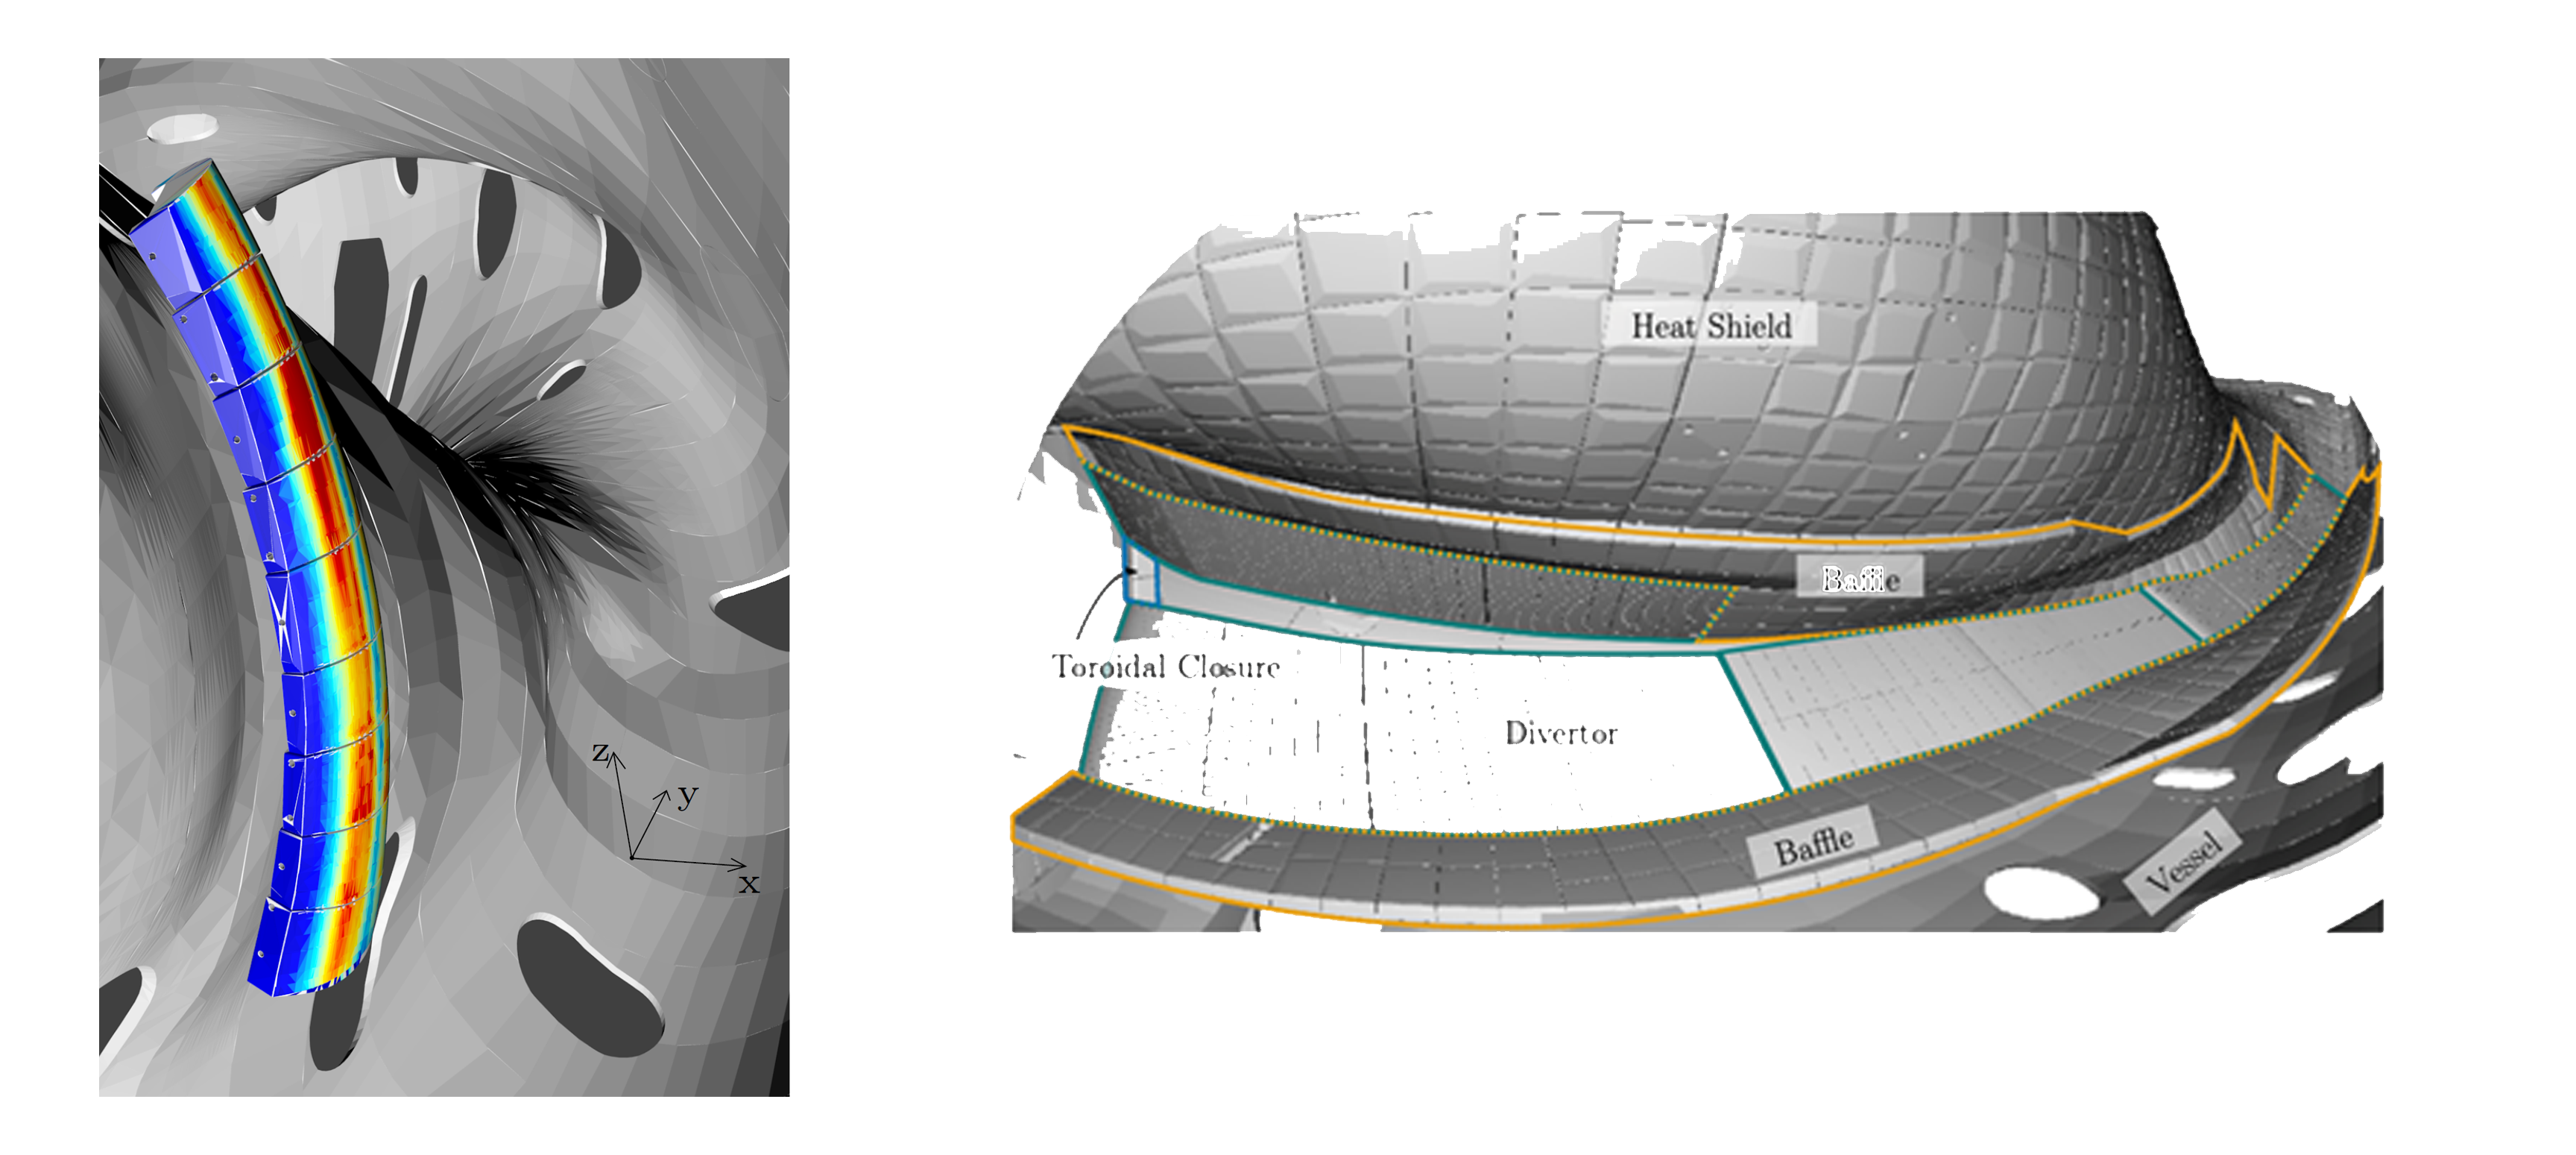
\includegraphics[width = \textwidth]{images/limiter-divetor.png}
    \caption{Left: Three-dimensional representation of the heat flux on the surface of a limiter in W7-X, taken from \cite{Böckenhoff_2018} Right: Labeled image of the OP1.2 divertor and plasma facing components} \label{fig:limiter-divertor}
\end{figure}

In the work from D. Böckenhoff et al., data was limited to 6 values of $I_B$ taken from actual experimental data. While they were able to reconstruct $I_B$ using only the real world data with an $rmse$ (root mean squared error) of 0.047 for the test set results when using interpolated and extrapolated data. $rmse$ is defined as:

\begin{equation}
    rmse = \sqrt{\frac{1}{n}\sum_{i=1}^{n}(y_i - \hat{y}_i)^2}
\end{equation}

However, the network did not perform as well when applied to extrapolated data. To improve the performance, the authors used synthetic data generated from simulated $\iota$-scan data to train a new version of the network. The validation set was also entirely synthetic. While the new network performed well, there was an observed systematic underestimation of $I_B$ by $-0.026 \pm 0.001$.

The best results came from using the neural network pretrained on synthetic data and trained on the real data set after. The combination yielded the best results, with an $rmse$ of 0.013 and better performance on extrapolated results overall.

\section{Blatzheim, 2018}
In the 2018 paper "Neural network performance enhancement for limited nuclear fusion experiment observations supported by simulations" from M. Blatzheim et al. \cite{Blatzheim_2018}, refined methods compared to those in the 2018 paper to improve the neural network performance are presented. The work presented in this paper also uses data from OP1.1 and a mix of measured and simulated inputs and outputs.

In this paper, several neural network architectures are compared: a fully connected feed-forward neural network with 3 layers of 64 notes each, a neural network composed of a series four 5x5, eight 3x3, and 16 more 3x3 convolutional filters followed by two fully connected layers, and a shallow network composed of an inception module, followed by pooling, a 1x1 convolutional layer, and two fully connected layers.

Different partitions of the input image were used. The input resolutions were $9x5$, $18x8$, $72x15$, $144x30$. Also, three different input parameterization of the partitions were tested: $(\mu, \sigma)$, $(\mu, \delta)$, and $\rho$. The $\mu$ and $\sigma$ parameterization is the standard deviation of the heat load, $\mu$ is the mean of the heat load, and $\delta$ is the difference between the maximum and minimum heat load values. The $\rho$ parameterization is the relative heat load. Increasing the number of inputs also resulted in a higher number of network parameters to accommodate the increased input size.

\begin{figure}[!htb]
    \centering
    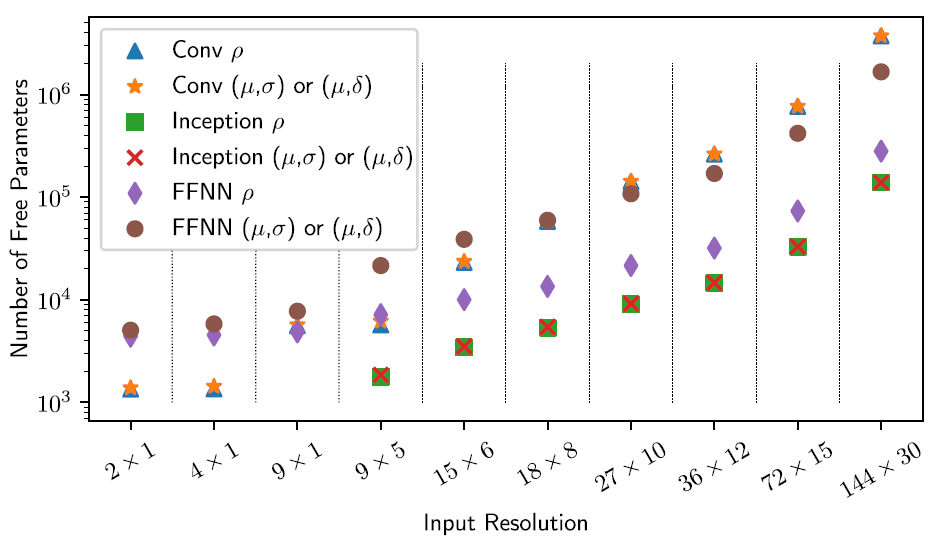
\includegraphics[width = \textwidth]{images/daniel-input-parameters.png}
    \caption{free parameters of the NN based on the input resolution, parameterization and architecture.} \label{fig:daniel-input-parameters}
\end{figure}

Solid results were found with the $9x5$ and $36x12$ resolutions using a convolutional NN and mixed real world and simulated data using the $\rho$ parameterization, achieving an $rmse$ of 0.008. The inception model showed improved performance for higher resolution inputs and could be useful for data like that from the OP1.2 campaign.

\section{Blatzheim, 2019}

The results from M. Blatzheim et al. were used as a baseline for the final paper in the series, "Neural Network Regression Approaches to Reconstruct Properties of Magnetic Configuration from Wendelstein 7-X Modeled Heat Load Patterns" \cite{Blatzheim_2019}. The authors used the results presented in the previous papers to improve the neural network performance, but unlike the prior papers which used data from the OP 1.1 campaign using a limiter, this paper looks at heat load data from the divertor that was added for the OP 1.2 campaign. Since this thesis is also using data from the OP 1.2 campaign, the results from this paper helped to inform the methods used in this thesis.

One of the issues with the dataset used in the work presented in the 2019 paper is that the reconstruction problem is more complex compared to the limiter configurations used for prior work. Despite the complexity, several neural architectures that performed well both in $rmes$ and with a 5-fold cross validation were produced. Good results were achieved with a convolutional neural network but the network was shallow compared to some of the deeper networks which tested better.